
\documentclass[a4paper,12pt]{article} % тип документа


% Русский язык
\usepackage[T2A]{fontenc} % кодировка
\usepackage[utf8]{inputenc} % кодировка исходного текста
\usepackage[russian,english]{babel} % локализация и переносы
\usepackage{graphicx}
\graphicspath{{pictures/}}
\DeclareGraphicsExtensions{.pdf,.png,.jpg}


% Математика
\usepackage{amsmath,amsfonts,amssymb,amsthm,mathtools}


\usepackage{wasysym}

%Заговолок
\author{Талашкевич Даниил Александрович}

\title{Лабораторная работа 1.4.5}

\date{\today}

\begin{document}

\maketitle
\thispagestyle{empty}

\newpage
\setcounter{page}{1}


{\bf 1. Аннотация}

В данной работе мы изучаем зависимость частоты колебаний струны от от величины ее натяжения, а также условия установления стоячей волны, получающейся в результате сложения волн,
идущих в противоположных направлениях

{\bf 2. Используемое оборудование}

Рейка со струной,звуковой генератор,постоянный магнит,разновесы.

{\bf 3. Теоретические сведения}

Струной в акустике называют однородную тонкую гибкую упругую нить.
Примерами могут служить сильно натянутый шнур или трос, струны гитары,
скрипки и других музыкальных инструментов. В данной работе изучаются
поперечные колебания стальной гитарной струны, натянутой горизонтально
и закрепленной между двумя неподвижными зажимами.
Основное свойство струны — гибкость — обусловлено тем, что её поперечные размеры малы по сравнению с длиной. Это означает, что напряжение
в струне может быть направлено только вдоль неё, и позволяет не учитывать
изгибные напряжения, которые могли бы возникать при поперечных деформациях (то есть, при изгибе струны)
.
В натянутой струне возникает поперечная упругость, т.е. способность сопротивляться всякому изменению формы, происходящему без изменения
объема. При вертикальном смещении произвольного элемента струны, возникают силы, действующие на соседние элементы, и в результате вся струна
приходит в движение в вертикальной плоскости, т.е. возбуждение «бежит» по
струне. Передача возбуждения представляет собой поперечные бегущие
волны, распространяющиеся с некоторой скоростью в обе стороны от места
возбуждения. В ненатянутом состоянии струна не обладает свойством поперечной упругости и поперечные волны на ней невозможны.

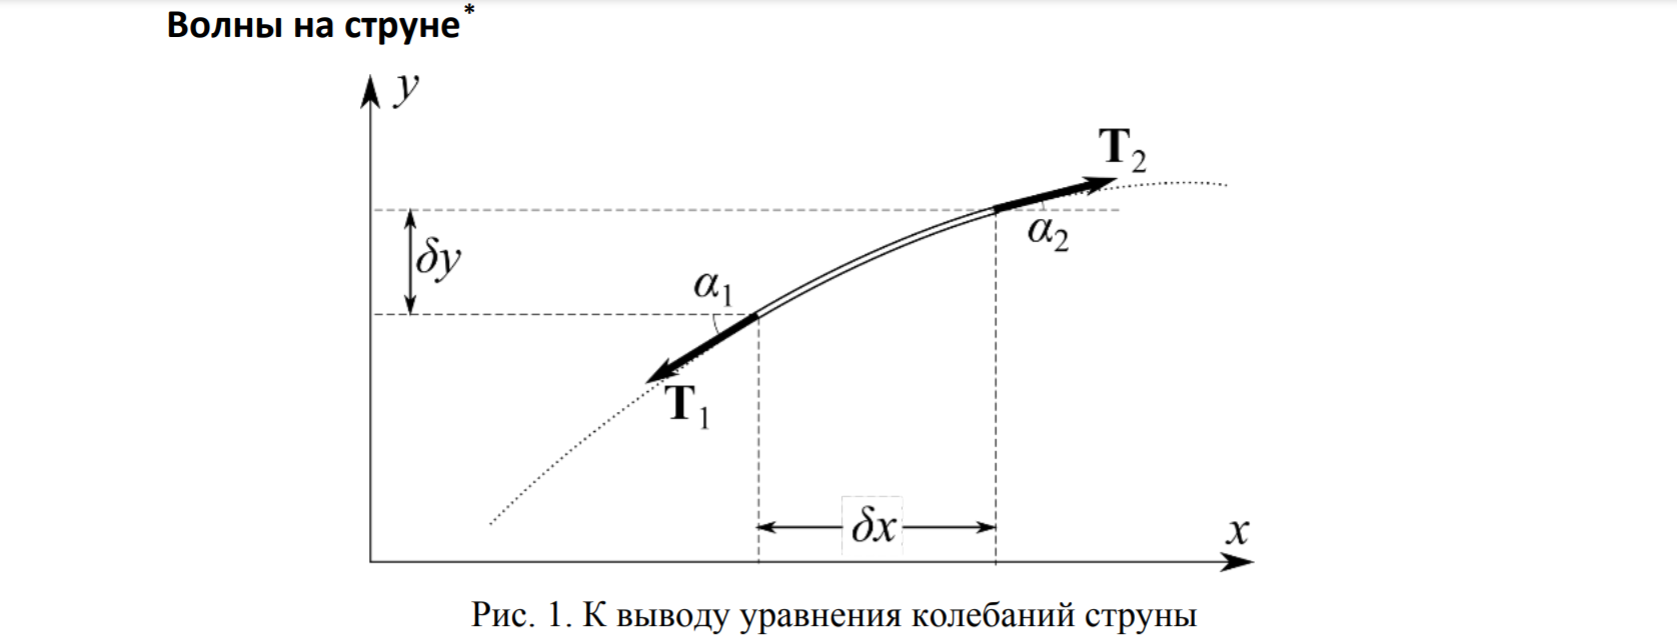
\includegraphics[width=\textwidth]{1.4.5 1}

Рассмотрим гибкую однородную струну, в которой создано натяжение $T$,
и получим дифференциальное уравнение, описывающее её малые поперечные свободные колебания. Отметим, что если струна расположена горизонтально в поле тяжести, величина $T$ должна быть достаточна для того, чтобы в
состоянии равновесия струна не провисала, т. е. сила натяжения должна существенно превышать вес струны.

Направим ось $x$ вдоль струны в положении равновесия. Форму струны будем описывать функцией $y (x,t)$, определяющей её вертикальное смещение в
точке $x$ в момент времени $t$ (см. рис. 1). Угол наклона касательной к струне в
точке $x$ относительно горизонтального направления обозначим как $\alpha$. В любой момент этот угол совпадает углом наклона касательной к графику функции $y(x)$ , то есть $\tg{\alpha} = \frac{\partial y}{\partial x}$.

Рассмотрим элементарный участок струны, находящийся в точке $x$, имеющий длину $\delta x$ и массу $\delta m = \rho_l \delta x$ , где $\rho_l	$ -- погонная плотность струны
(масса на единицу длины). При отклонении от равновесия на выделенный
элемент действуют силы натяжения $T_1$ и $T_2$, , направленные по касательной к
струне. Их вертикальная составляющая будет стремиться вернуть рассматриваемый участок струны к положению равновесия, придавая элементу некоторое вертикальное ускорение $\frac{\partial^2{y}}{\partial{t^2}}$.Заметим, что угол $\alpha$ зависит от координаты
$x$ вдоль струны и различен в точках приложения сил $T_1$ и $T_2$. Таким образом,
второй закон Ньютона для вертикального движения элемента струны запишется в следующем виде: 

\[ \delta m\frac{\partial^2{y}}{\partial{t^2}} = -T_1\sin{\alpha_1} + T_2\sin{\alpha_2} .\]

Основываясь на предположении, что отклонения струны от положения
равновесия малы, можем сделать ряд упрощений:

1. Длина участка струны в изогнутом состоянии практически равна
длине участка в положении равновесия
, поэтому добавочным напряжением вследствие удлинения струны можно пренебречь. Следовательно, силы $T_1$ и $T_2$ по модулю равны силе натяжения струны: $T_1 \approx T_2 \approx T.$

2. Углы наклона $\alpha$ малы, поэтому $\tg{\alpha} \approx \sin{\alpha} \approx \alpha$.

Разделим обе части уравнения движения на $\delta x$ и устремим размер элемента к нулю, $\delta x$ → 0. Тогда правая часть примет вид

\[ \rho_l \frac{\partial^2{y}}{\partial{t^2}} = \frac{T_2 \sin{\alpha_2} - T_1 \sin{\alpha_1}}{\delta x} \approx T \frac{\alpha_2 - \alpha_1}{\delta x} \rightarrow T\frac{\partial{\alpha}}{\partial{x}}. \]

(в последнем переходе использовано определение производной функции как
предела отношения приращения функции к приращению аргумента). Наконец, подставляя $\alpha = \frac{\partial y}{\partial x}$, и вводя обозначение 


\[ u = \sqrt{\frac{T}{\rho_l}} .\]

что, как мы увидим далее, есть скорость распространения волн на струне,
находим окончательно уравнение свободных малых поперечных колебаний
струны:

\[  \frac{\partial^2 y}{\partial t^2} = u^2\frac{\partial^2 y}{\partial x^2} .\]

Это уравнение называют волновым уравнением. Кроме волн на струне, оно
может описывать волновые процессы в самых разных системах, в том числе
волны в сплошных средах (звук), электромагнитные волны и т.д.

Еще из важных формул :

1) Частота через омегу \[ \nu = \frac{\omega}{2\pi}.\]

2) Длина струны \[ L = \frac{\lambda_n}{2}n .\]

3) И, наконец, возможные частоты колбеания струны \[ \nu_n = \frac{u}{\lambda_n} = \frac{n}{2L} \sqrt{\frac{T}{\rho_l}} .\]

Набор (спектр) разрешённых частот $\nu_n$ называют собственными частотами
колебаний струны. Режим колебаний, соответствующий каждой из частот $\nu_n$,
называется собственной (или нормальной) модой колебаний (от англ. $mode$ —
режим). Произвольное колебание струны может быть представлено в виде суперпозиции её собственных колебаний. Наименьшая частота $\nu_1$ называется
также основным тоном (или первой гармоникой), а остальные ($\nu_2$ = $2 \nu_1$, $\nu_3 = 3\nu_1$,$\dots$) — обертонами (высшими гармониками). Термин «гармоника» иногда
употребляется в обобщенном смысле — как элементарная составляющая
сложного гармонического колебания.

На Рис. 2 показана картина стоячих волн для $n = 1, 2, 3$ . Заметим, что
число $n$ определяет число пучностей (но не узлов!) колеблющейся струны.
Таким образом, спектр собственных частот струны определён её погонной
плотностью $\rho_l$, силой натяжения $T$ и длиной струны $L$ (отдельно отметим, что
собственные частоты не зависят от модуля Юнга материала струны).

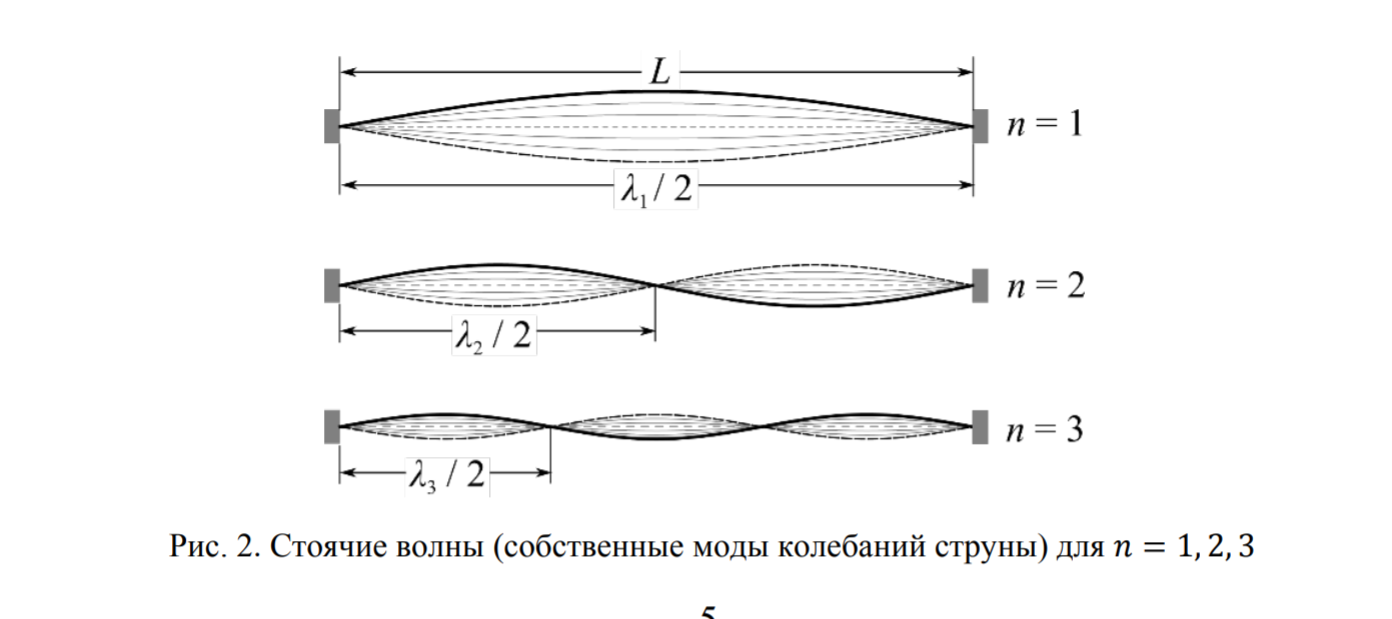
\includegraphics[width=\textwidth]{1.4.5 3}

{\bf Экспериментальная установка}

Схема установки приведена на Рис. 3. Стальная гитарная струна 1 закрепляется в горизонтальном положении между двумя стойками с зажимами 2 и 3,
расположенными на массивной станине 4. Один конец струны закреплен в
зажиме 2 неподвижно. К противоположному концу струны, перекинутому через блок, прикреплена платформа с грузами 5, создающими натяжение
струны. Зажим 3 можно передвигать по станине, устанавливая требуемую
длину струны. Возбуждение и регистрация колебаний струны осуществляются с помощью электромагнитных датчиков (вибраторов), расположенных
на станине под струной. Электромагнитный датчик 6 подключен к звуковому
генератору 7 и служит для возбуждения колебаний струны, частота которых
измеряется с помощью частотомера 10 (в некоторых установках частотомер
встроен в генератор). Колебания струны регистрируются с помощью электромагнитного датчика 8, сигнал с которого передается на вход осциллографа 9.
Разъёмы, через которые датчики с помощью кабелей соединяются с генератором и осциллографом, расположены на корпусе станины.

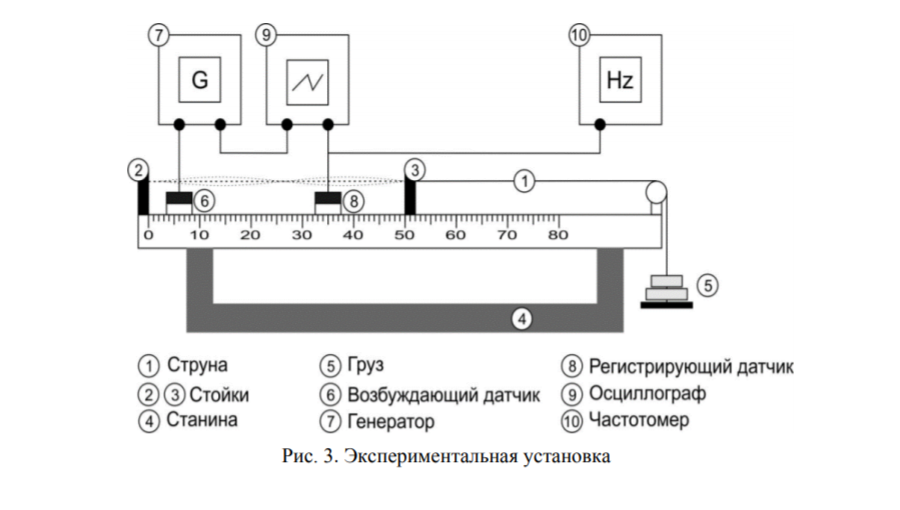
\includegraphics[width=\textwidth]{1.4.5 4}

{\bf Принцип работы датчиков}

Устройство и внешний вид электромагнитного датчика показаны на Рис. 4.
В пластмассовом корпусе датчика закреплен подковообразный магнит. На полюсах
магнита намотаны соединенные последовательно катушки переменного тока, который подается с генератора. Магнитное
поле в зазоре между полюсами электромагнита складывается из поля постоянного
магнита $B_0$ и малой добавочной составляющей поля катушек $B_{\sim} \ll B_0$ . Сила, с которой электромагнит действует на стальную
(магнитную) струну, пропорциональна
квадрату индукции B суммарного поля в
зазоре электромагнита :

\[ F\propto (B_0+ B_{\sim})^2 \approx B_0^2 + 2B_0B_{\sim} .\]

\begin{center}
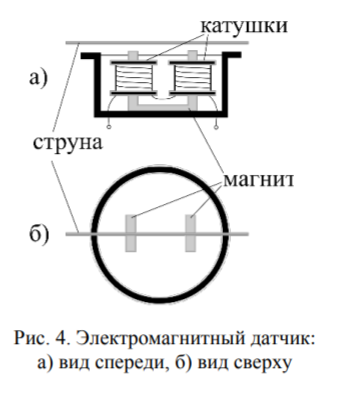
\includegraphics[scale=0.8]{1.4.5 5}
\end{center}

Отсюда видно, что при $B_{\sim} \ll B_0$ сила $F$ линейно зависит от переменного
поля$B_{\sim}$ , а значит и от тока в катушках (т. к. $B_{\sim}  \propto I_{\sim}$), и поэтому частота переменой силы $ F_{\sim} \propto I_{\sim}$ , действующей на струну, совпадает с частотой генератора. То есть участок струны, расположенный над электромагнитом, совершает колебательное движение в вертикальной плоскости с частотой задающего генератора. Колебания далее передаются по всей струне и,
если частота колебаний совпадает с одной из собственных частот струны, на
струне устанавливается стоячая волна. Колеблющаяся струна возбуждает в
регистрирующей катушке переменную ЭДС с амплитудой, пропорциональной амплитуде колебаний струны. Сигнал ЭДС измеряется с помощью осциллографа.
Отметим, что магнитное поле наиболее однородно по координате в центральной части электромагнита, поэтому датчики должны быть повернуты
так, чтобы струна располагалась в центральной части перпендикулярно к полюсам магнита. Возбуждающий датчик следует расположить вблизи неподвижного конца струны (ближе к узлу), а регистрирующий — в пучности.

{\bf Измерения с помощью осциллографа}

Для регистрации колебаний струны в работе используется электронный
осциллограф, соединённый с электромагнитным датчиком 8. Он позволяет
регистрировать колебания в случаях, когда это невозможно сделать визуально. Также с помощью осциллографа можно измерять амплитуду возбуждения и форму сигнала, что даёт возможность установить, является ли режим
возбуждения стоячих волн линейным, иными словами, имеет ли место прямая пропорциональность между силой возбуждения и амплитудой колебаний
струны, и не возникает ли отклонений от закона. 

Контролировать величину и форму сигнала колебаний струны на экране
осциллографа можно несколькими способами: в одноканальном (переключатель $MODE$ в положении $CH2$) и двухканальном (переключатель $MODE$ в положении $DUAL$) режимах работы осциллографа — по временной развертке
сигналов, а также в режиме сложения двух взаимно перпендикулярных сигналов — основного и опорного (режим $X$--$Y$).

При возбуждении стоячей волны на экране осциллографа в режиме развертки должен появиться сигнал синусоидальной формы. При чрезмерном
возбуждении вид синусоиды искажается, что свидетельствует об отклонении
от линейного режима. В двухканальном режиме осциллографа можно сравнить опорный (подаваемый одновременно на возбудитель колебаний 6 и канал CH1 осциллографа) и основной (снимаемый с датчика 8) сигналы — в
отсутствие нелинейных искажений они должны совпадать. Кроме того, в режиме сложения сигналов (X–Y) на экране должен прорисовываться эллипс
правильной формы.

Дополнительным критерием того, что частота гармоники определена
верно, является симметричность «резонансной кривой» — амплитудно-частотной характеристики системы (Рис. 5). А именно, при подходе к резонансной частоте со стороны как высоких, так и со стороны низких частот, максимум сигнала наблюдается при одном и том же значении частоты.

\begin{center}
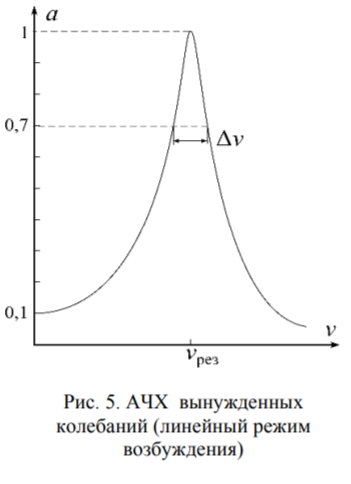
\includegraphics[scale=0.8]{1.4.5 6}
\end{center}








\newpage

{\bf ХОД РАБОТЫ}
\\

{\bf Установка грузов} 

Освобождаем зажим струны на стойке 3, установить длину струны $L = 50$ см. Натянем струну, поставив на платформу грузы ($F \approx 1$ кг), с учетом веса платформы и крепежа. Осторожно зажмем струну в стойке, не деформируя струну. В свою очередь возбуждающий датчик 6 должен располагаться рядом с неподвижной
стойкой 2, т.е. вблизи узла стоячей волны.

{\bf Предварительные расчеты}

Оценитваем скорость распространения волн, используя табличное значение плотности стали и
приняв диаметр струны равным $d \approx 0,3$ мм. Для заданных значений длины
струны и силы натяжения рассчитайте частоту основной гармоники $\nu_1$.

{\bf Определение $\nu_1$}

Медленно меняя частоту звукового генератора в диапазоне $\nu = \nu_1 \pm 5 \textbf{ Гц }$ добиваемся возбуждения стоячей волны на основной гармонике (одна пучность). Если при колебаниях струна касается регистрирующего датчика 8,
осторожно сдвигаем датчик по скамье в сторону подвижного зажима
струны 3. Определяем частоту первой гармоники по частотомеру. Далее увеличиваем частоту, чтобы получить картину стоячих волн на второй
гармонике, а затем и на более высоких гармониках.

Настраиваем осциллограф нужным образом и переходим к следующей части.

{\bf  Регистрация стоячих волн с помощью осциллографа}

При пяти различных силах натяжения снимаем данные о частотах (не менее 5 для нечетных и столько же для четных). При этом длина струны $L \approx 50\textbf{см }$,а для четных частот нужно смещать регистрирующий датчик 8 по станинев предварительно рассчитаные положения пучностей. А так же во избежание взаимного влияния («резонирования») датчиков регистрирующий датчик следует сдвигать в строну подвижного зажима струны 3. 



{\bf Таблицы полученных данных}

Для дальнейших измерений силы натяжения будем использовать формулу \[ T = (M + m_i)g.\]

Где $M$ -- масса установки (платформы и ключка), а $m_i$ -- масса подвешенных грузиков, котоую мы изменяем на протяжении эксперимента.



\newpage
{\bf Таблицы :}\\

\begin{center}

\begin{tabular}{|c|c|c|c|c|c|c|c|c|c|c|}
\hline 
\multicolumn{11}{|c|}{$\textbf{Натяжение } T_1 = 10,5H$ } \\ 
\hline 
$n=$ & $1$ & $2$ & $3$ & $4$ & $5$ & $6$ & $7$ & $8$ & $9$ & $\nu_1(\textbf{теор.})$\\ 
\hline 
$\nu=$ & $134,5$ & $270$ & $407,5$ & $543,3$ & $680,3$ & $815,3$ & $957,1$ & $1086,4$ & $1236,4$ & $136$\\
\hline
$U = $ & $134,5$ & $135$ & $135,8$ & $135,8$ & $136,1$ & $135,9$ & $136,7$ & $135,8$ & $137,4$ & $\overline{U} = 135,9$\\

\hline 
\end{tabular} 

\end{center}

\begin{center}

\begin{tabular}{|c|c|c|c|c|c|c|c|c|c|c|}
\hline 
\multicolumn{11}{|c|}{$\textbf{Натяжение } T_2 = 15,3 H$ } \\ 
\hline 
$n=$ & $1$ & $2$ & $3$ & $4$ & $5$ & $6$ & $7$ & $8$ & $9$ & $\nu_1(\textbf{теор.})$\\ 
\hline 
$\nu=$ & $162,6$ & $327,3$ & $491,4$ & $656$ & $821,2$ & $986,3$ & $1152,1$ & $1319,7$ & $1485,9$ & $164$\\ 
\hline
$U = $ & $162,6$ & $163,7$ & $163,8$ & $164$ & $164,2$ & $164,4$ & $164,6$ & $165$ & $165,1$ & $\overline{U}= 164,2$\\

\hline 
\end{tabular} 

\end{center}

\begin{center}

\begin{tabular}{|c|c|c|c|c|c|c|c|c|c|c|}
\hline 
\multicolumn{11}{|c|}{$\textbf{Натяжение } T_3 = 20,1 H$ } \\ 
\hline 
$n=$ & $1$ & $2$ & $3$ & $4$ & $5$ & $6$ & $7$ & $8$ & $9$ & $\nu_1(\textbf{теор.})$\\ 
\hline 
$\nu=$ & $187,1$ & $376,4$ & $563,8$ & $752$ & $941,3$ & $1130,9$ & $1320,5$ & $1511,7$ & $1702,7$ & $188$\\
\hline
$U = $ & $187,1$ & $188,2$ & $187,9$ & $188$ & $188,3$ & $188,5$ & $188,6$ & $189$ & $189,2$ & $\overline{U} = 188,3$\\
\hline 
\end{tabular} 

\end{center}

\begin{center}

\begin{tabular}{|c|c|c|c|c|c|c|c|c|c|c|}
\hline 
\multicolumn{11}{|c|}{$\textbf{Натяжение } T_4 = 25 H$ } \\ 
\hline 
$n=$ & $1$ & $2$ & $3$ & $4$ & $5$ & $6$ & $7$ & $8$ & $9$ & $\nu_1(\textbf{теор.})$\\ 
\hline 
$\nu=$ & $208,9$ & $419,2$ & $628,5$ & $838,6$ & $1048,7$ & $1259,1$ & $1468$ & $1676,8$ & $1893$ & $209,8$\\
\hline
$U = $ & $208,9$ & $209,6$ & $209,5$ & $209,7$ & $209,7$ & $209,9$ & $209,7$ & $209,6$ & $210,3$ & $\overline{U} = 209,7$\\
\hline 
\end{tabular} 

\end{center}
{\bf Обработка результатов измерений 1. Сравнение значений частот}

Полученные значения очень близки к теоретическим, потому что законы, описывающие поведение струны, очень точны, а так же погрешность измерений крайне мала ввиду высокой точности осциллографа, генератора частот.

{\bf *}
Благодаря высокой добротности струны, возможно возбуждение её
колебаний при кратных частотах генератора, меньших, чем $\nu_1$. Для наблюдения явления переключаем осциллограф в режим ($X$--$Y$) и настраиваем установку
на наблюдение основной гармоники. Затем уменьшите частоту возбуждения
в два раза, установив на генераторе $\nu$ = $\nu_1/2$.На экране осциллографа должна
наблюдаться фигура Лиссажу с одним самопересечением. вот, что вышло у меня в данном эксперименте:

\begin{center}
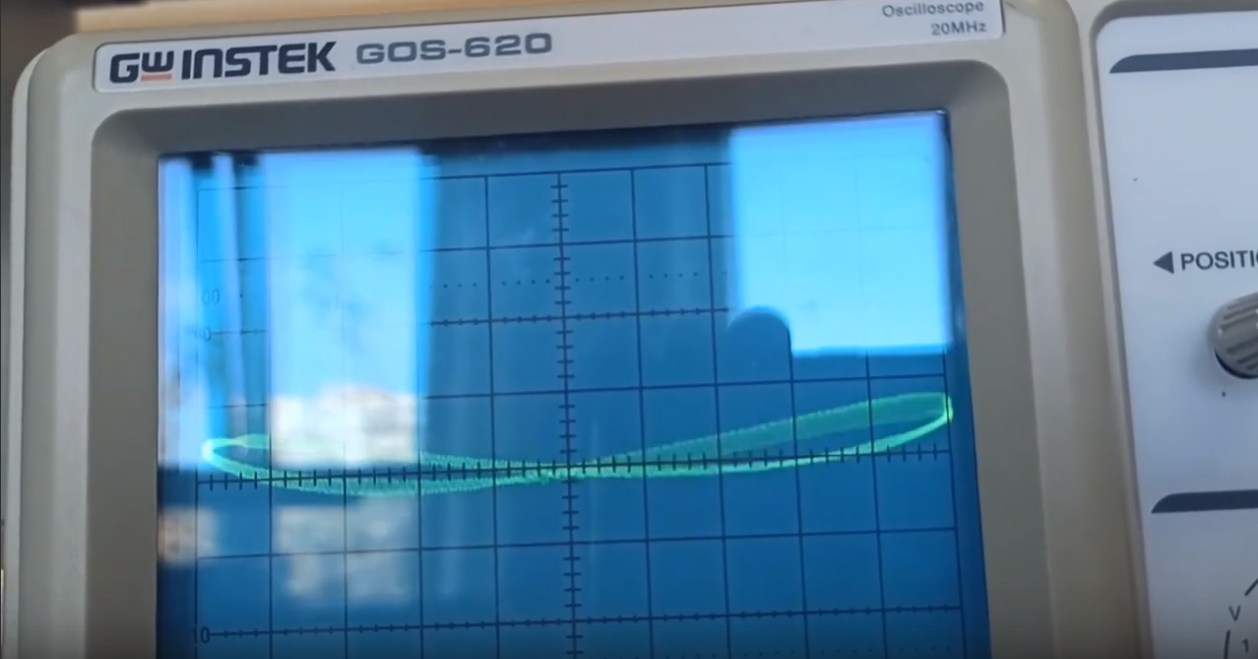
\includegraphics[scale=0.6]{1.4.5 7}
\end{center}

Схематически фигура Лиссажу имеет вид близкий к этому:

\begin{center}
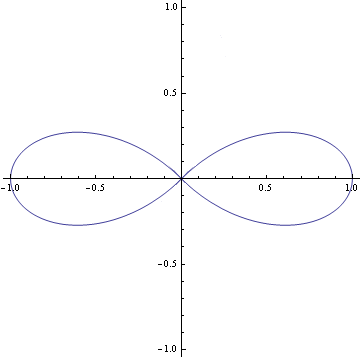
\includegraphics[scale=0.85]{1.4.5 8}
\end{center}

{\bf Определение добротности $Q$ струны как колебательной системы}

Измерив её амплитудно-частотную характеристику (АЧХ) вблизи одной из резонансных частот (в качестве таковых выбрана $\nu_3$).

Для расчётов воспользуфемся известным из теории колебаний результатом:
добротность колебательной системы связана с резонансной частотой $\nu_{\textbf{рез}}$ и шириной резонансной кривой $\bigtriangleup \nu$ соотношением \[ Q = \frac{\nu_{\textbf{рез}}}{\bigtriangleup \nu} . \]

где ширина резонансной кривой $\bigtriangleup \nu$ измеряется на уровне амплитуды, составляющей 0,7 от амплитуды в резонансе
(Рис. 5).






\begin{center}
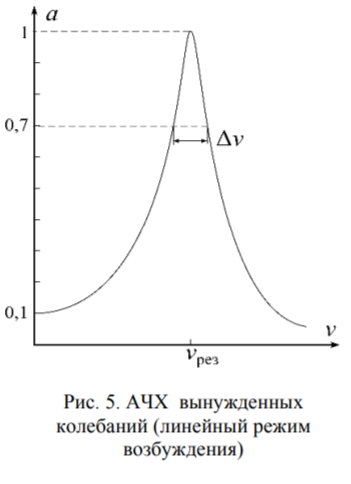
\includegraphics[scale=0.8]{1.4.5 6}
\end{center}

По формуле получим, что добротность $Q$ струны как колебательной системы равна $Q \approx \dots$

{\bf Обработка результатов измерений 2.}

Графики зависимости $\nu_n(n)$ для различных $T$ :

\begin{center}
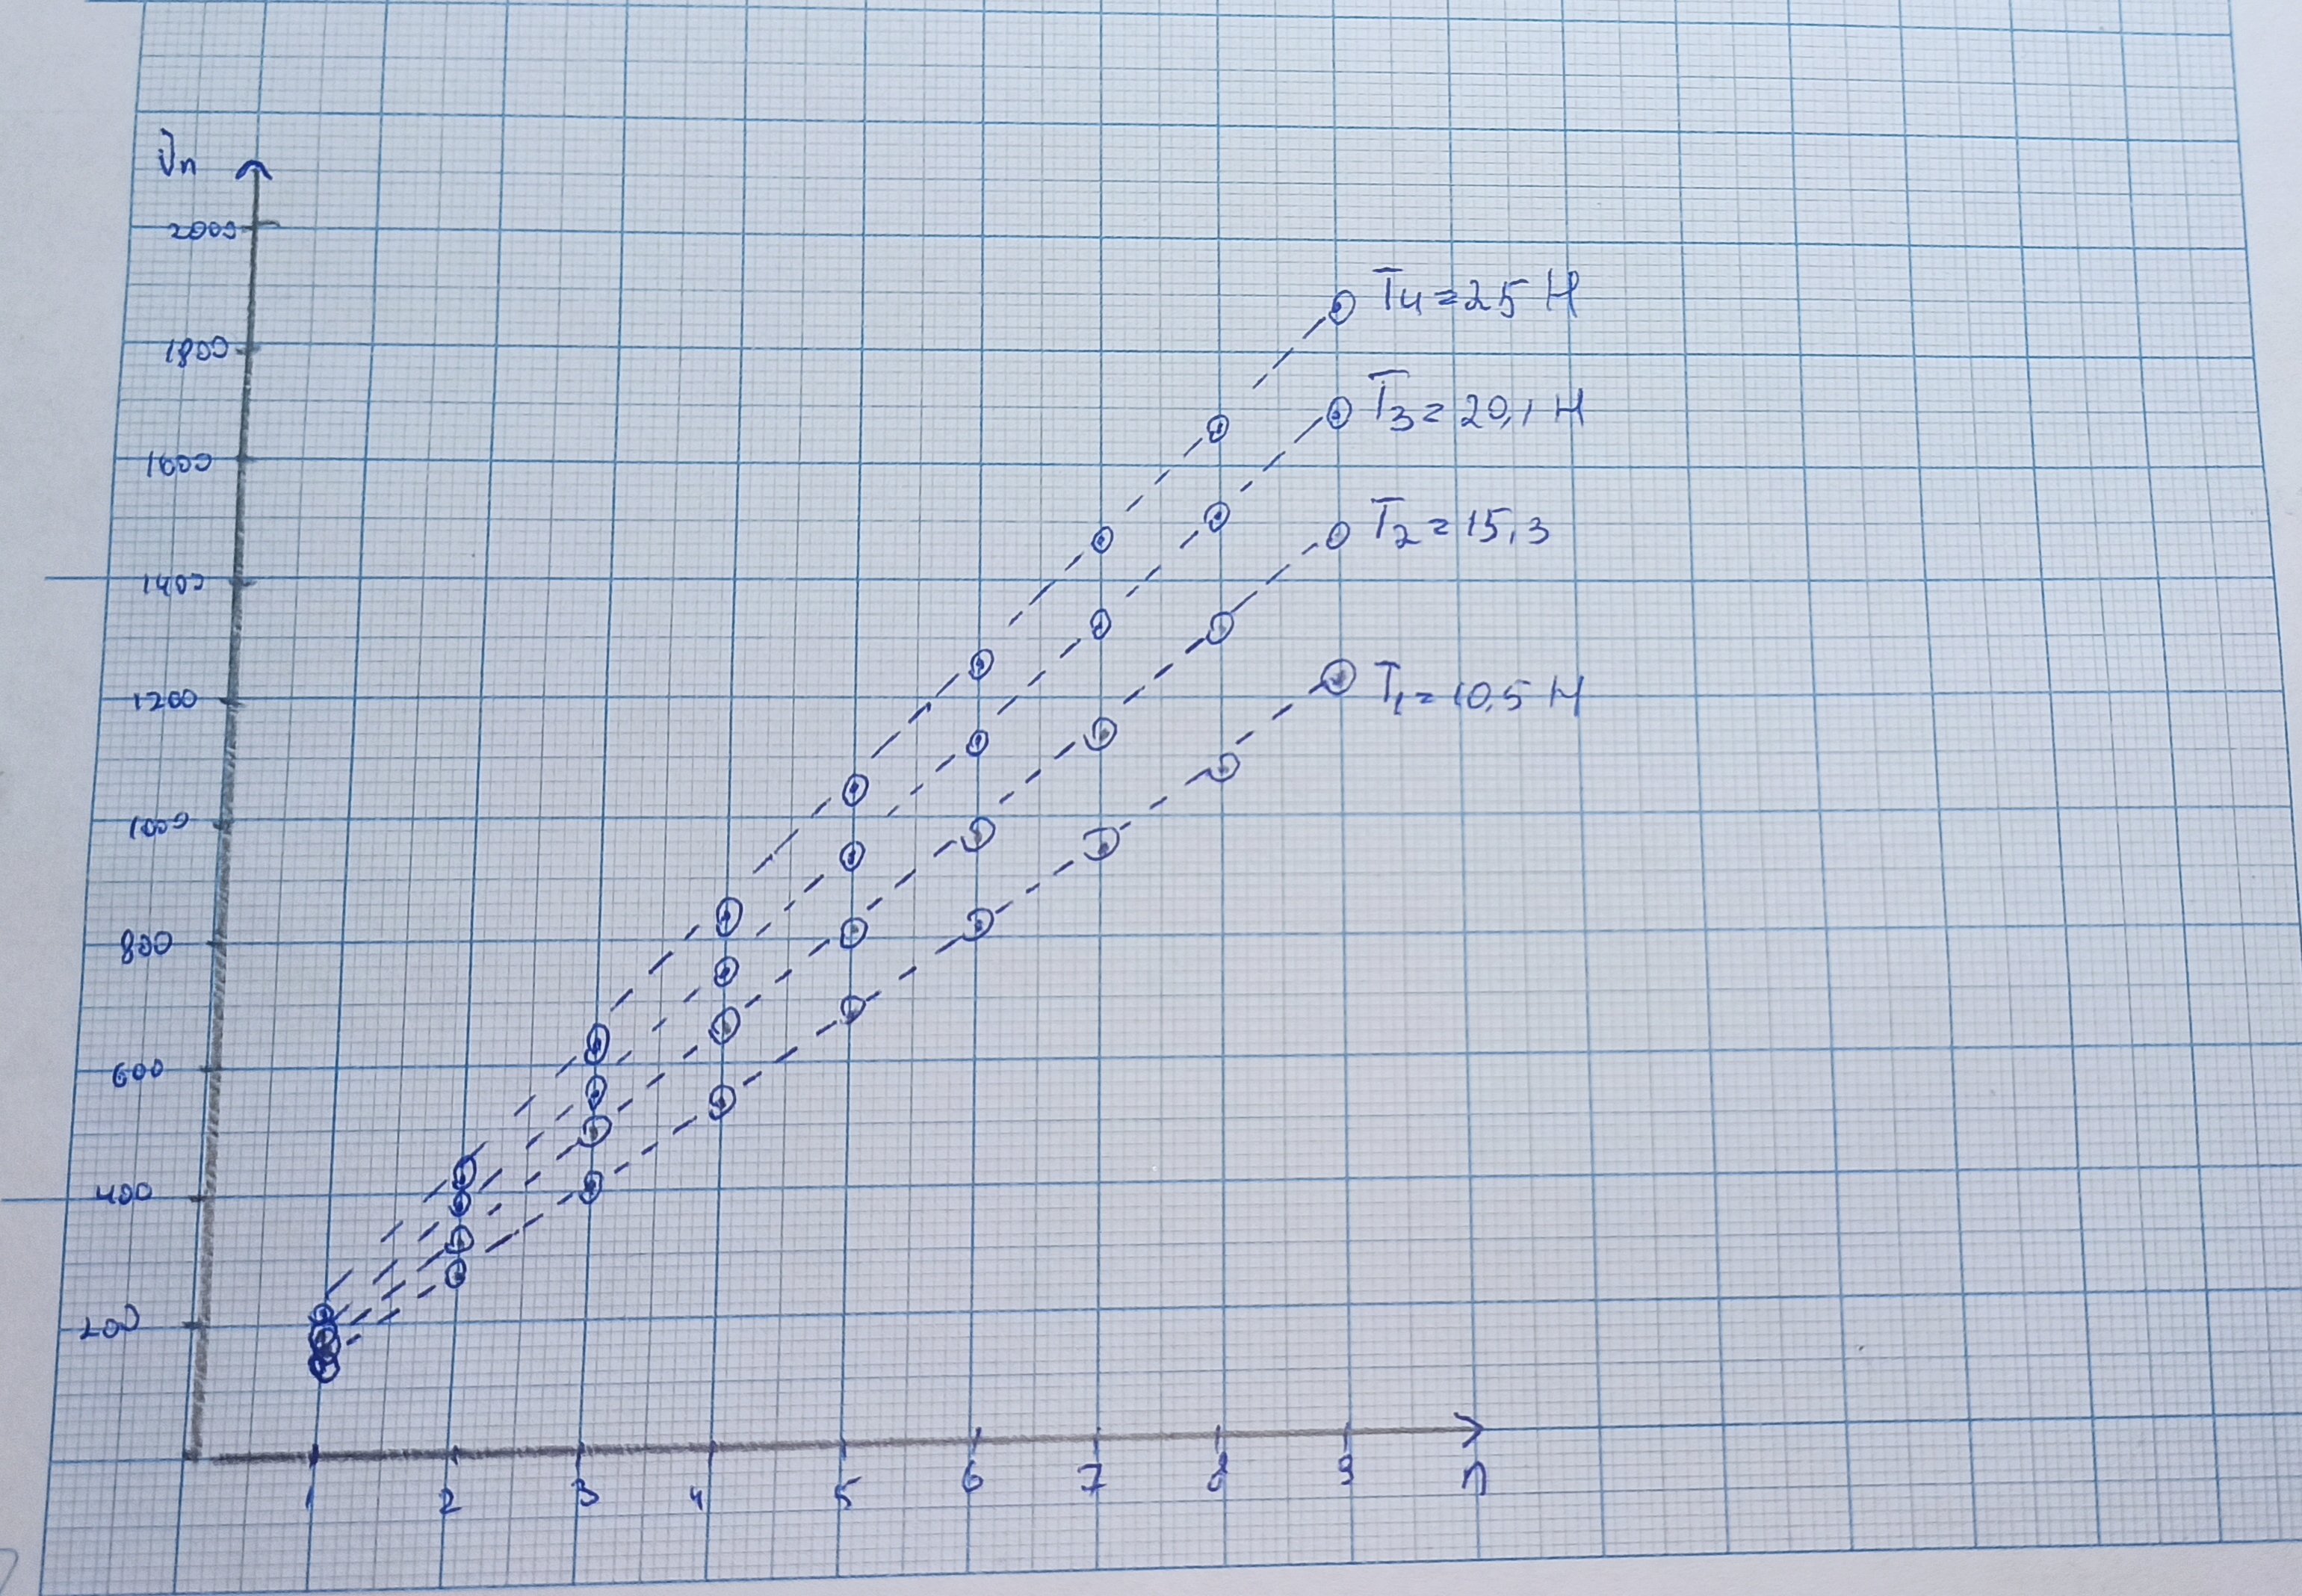
\includegraphics[scale=0.17]{1.4.5 9}
\end{center}

Определим среднее значение $\overline{u}$, при различных силах натяжения $T$ методом наименьших квадратов.

 \[ \sigma_{\overline{u}} = \sqrt{\frac{\sum\limits_{i = 1}^{N = 9}(u_i-\overline{u})^2}{N(N-1)}} \]
 
Построим таблицу расчитанных значений погрешностей:
\begin{center}

\begin{tabular}{|c|c|c|c|}
\hline 
$T$, H & $\overline{u}\textbf{,} \frac{\textbf{м}}{\textbf{с}}$ & $\sigma_{\overline{u}}\textbf{,} \frac{\textbf{м}}{\textbf{с}}$ & $\epsilon_{u}, \% $ \\ 
\hline 
$10,5$ & 135,9 & 0,28 & 0,21 \\ 
\hline 
$15,3$ & 164,2 & 0,25 & 0,15 \\ 
\hline 
$20,1$ & 188,3 & 0,2 & 0,11 \\ 
\hline 
$25$ & 209,7 & 0,12 & 0,06 \\ 
\hline 
\end{tabular}

\end{center} 

{\bf Обработка результатов измерений 3. Постройте график зависимости квадрата скорости $u^2$ от силы натяжения
$T$}

Построим таблицу $u^2(T)$, построим график полученной зависимости и определим погонную плотность струны $\rho_l$ и оценим погрешность результата. И в заключение сравним полученное значение со значением, указанным на установке.

\begin{tabular}{|c|c|}
\hline 
$u^2$, м$^2$ /c$^2$ & $T$, c \\ 
\hline 
18469 & 10,5 \\ 
\hline 
26962 & 15,3 \\ 
\hline 
35457 & 20,1 \\ 
\hline 
43974 & 25 \\ 
\hline 
\end{tabular} 

Соответственно график $u^2(T)$ :

\begin{center}
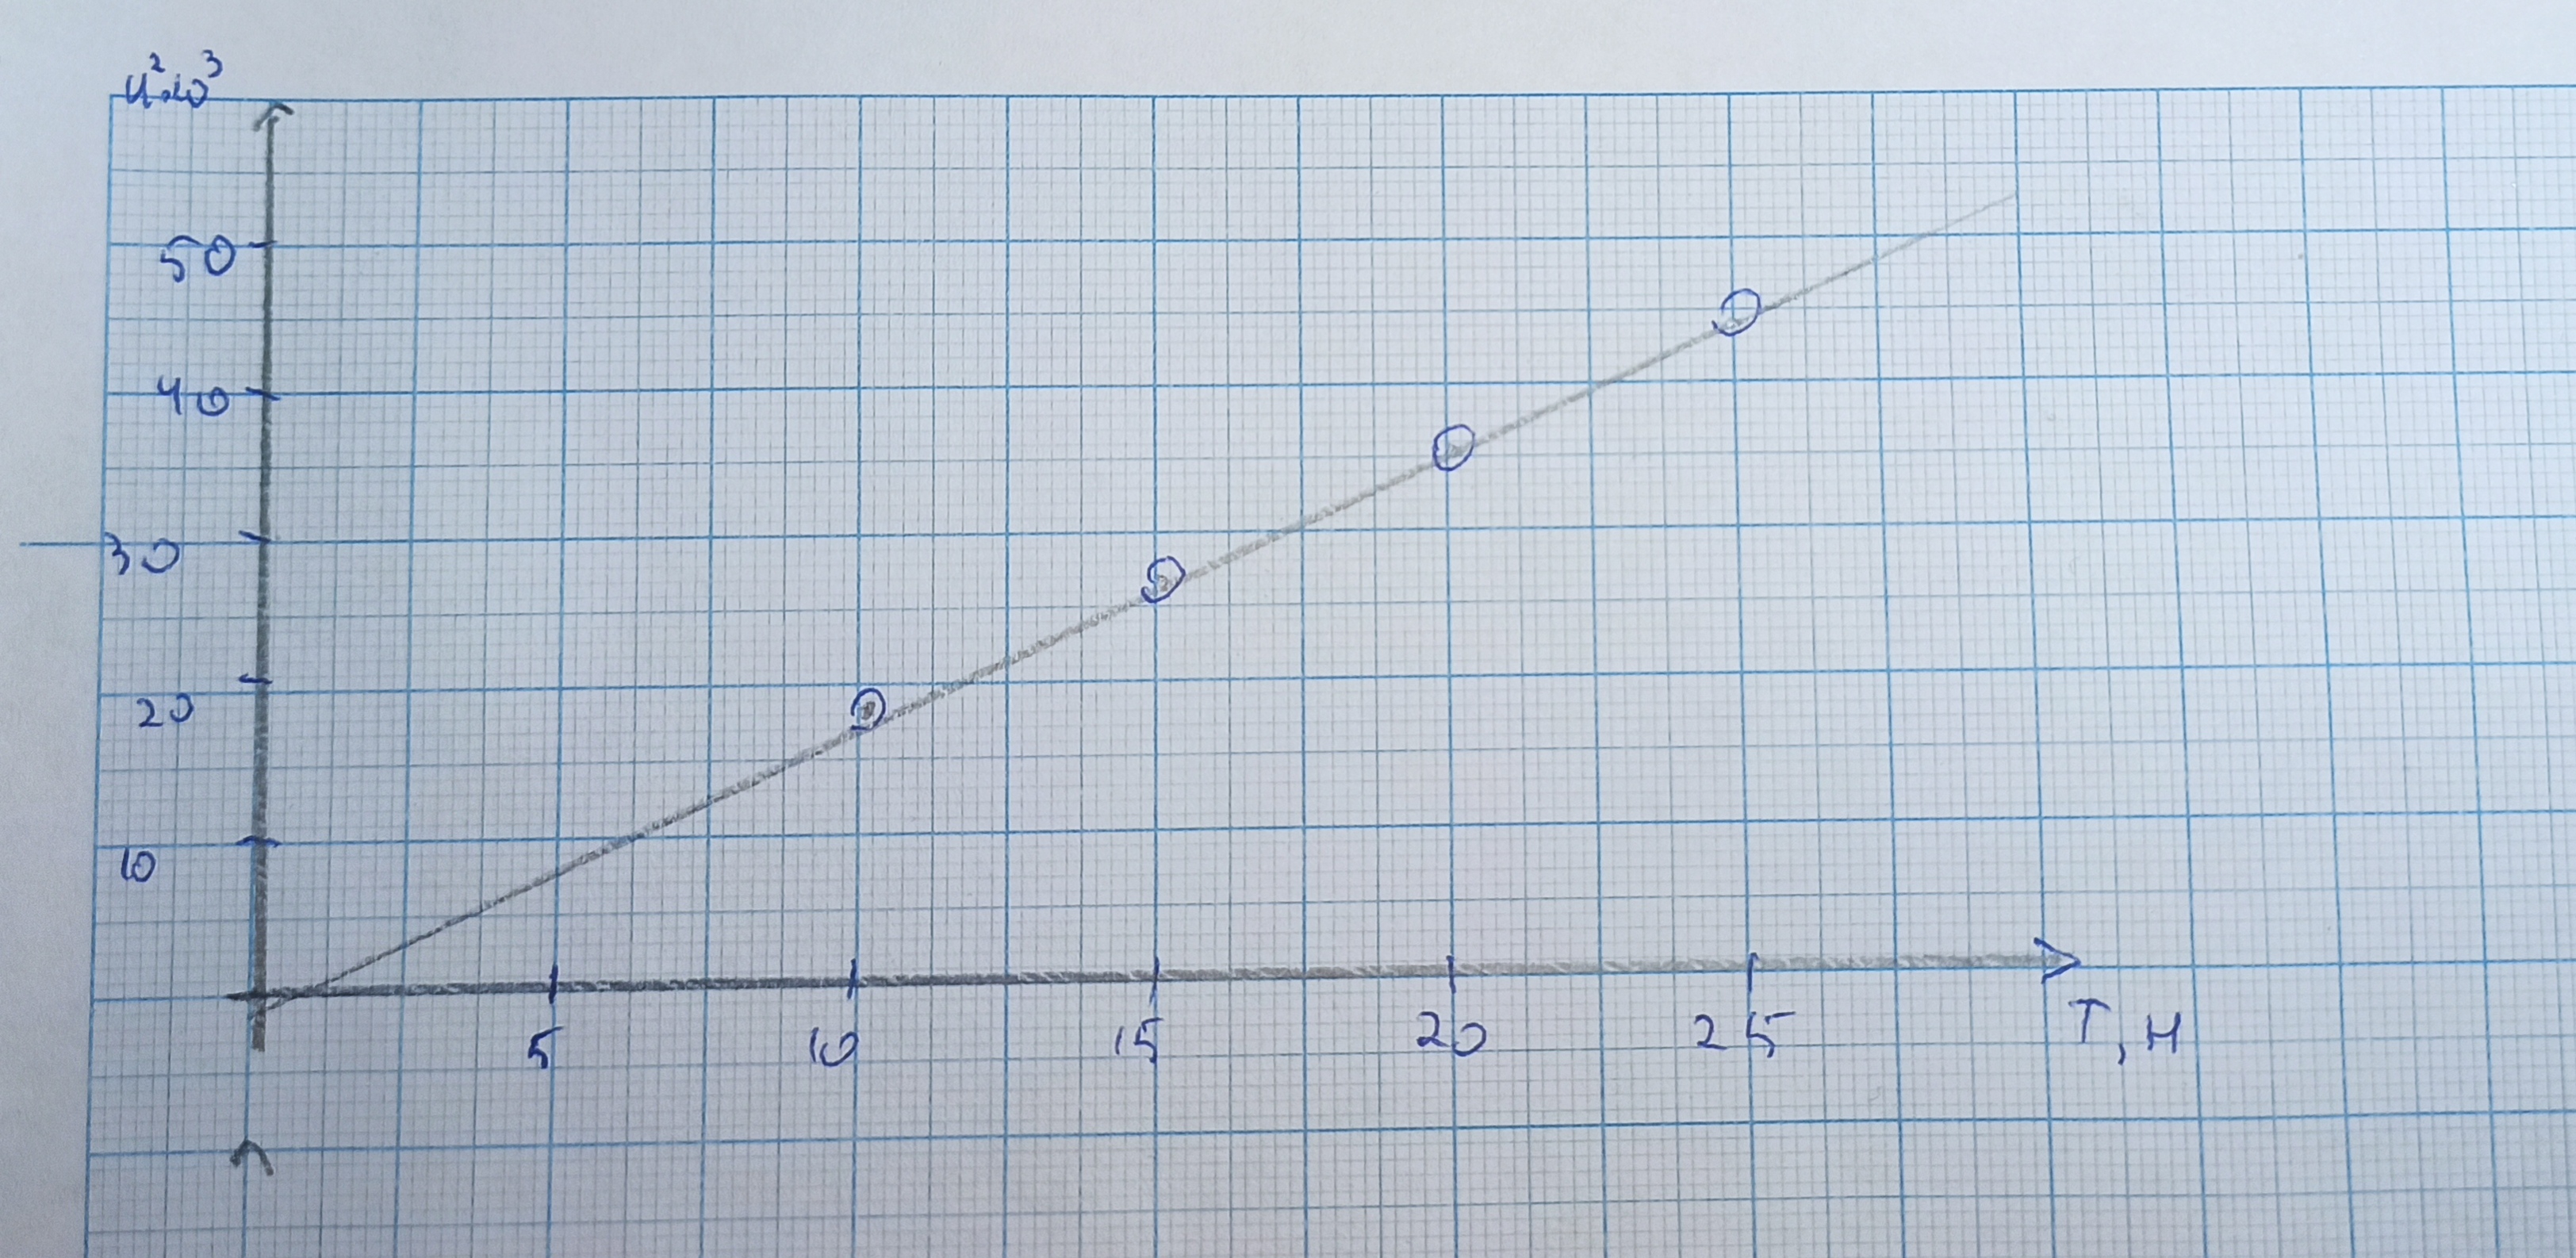
\includegraphics[scale=0.15]{1.4.5 10}
\end{center}

Расчет по графику дает : $\rho_l \approx 568,5\cdot 10^{-6}$.

Расчет по методу МНК :  $\rho_l \approx 568,45 \cdot 10^{-6} \pm 0,02\cdot 10^{-6}$.

Значение на установке : $\rho_l = 568,4 \cdot 10^{-6}$.

Полученное значение идентично со значение, указанным на установке.







{\bf Вывод : }

Экспериментальным путем изучили поперечные стоячие волны на струне, научились определять собственные частоты колебаний струны, исследовали зависимость скорости распространения поперечныз волн на струне в зависимости от ее натяжения. Экспериментальным путем с почти идеальной точностью нашли значение погонной плотность струны $ \rho_l$ и оценили погрешность результата. А так же закрепили уже имевшийся опыт работы с осциллографом и генератором частот.










${\bf }$









\end{document}


